% *********************************************************************
% © 2010–2022 Jeremy Sylvestre
%
% Permission is granted to copy, distribute and/or modify this document
% under the terms of the GNU Free Documentation License, Version 1.3 or
% any later version published by the Free Software Foundation; with no
% Invariant Sections, no Front-Cover Texts, and no Back-Cover Texts. A
% copy of the license is included in the appendix entitled “GNU Free
% Documentation License” that appears in the output document of this
% PreTeXt source code. All trademarks™ are the registered® marks of
% their respective owners.
%
% *********************************************************************

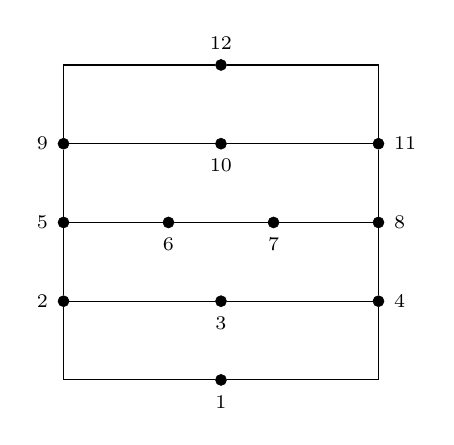
\begin{tikzpicture}[
	vertex/.style={ circle, draw, very thin, fill, inner sep=0pt, minimum size=4pt },
	vertexg/.style={ black!40!white, circle, draw, very thin, fill, inner sep=0pt, minimum size=4pt },
	vertexo/.style={ circle, draw, very thin, inner sep=0pt, minimum size=4pt }
]

\node at (0,0) (v1) [vertex,label=below:$\scriptstyle 1$] {};

\node at (-2,1) (v2) [vertex,label=left:$\scriptstyle 2$] {};
\node at (0,1) (v3) [vertex,label=below:$\scriptstyle 3$] {};
\node at (2,1) (v4) [vertex,label=right:$\scriptstyle 4$] {};
\draw (v1) to (-2,0) to (v2) to (v3) to (v4) to (2,0) to (v1);

\node at (-2,2) (v5) [vertex,label=left:$\scriptstyle 5$] {};
\node at (-0.667,2) (v6) [vertex,label=below:$\scriptstyle 6$] {};
\node at (0.667,2) (v7) [vertex,label=below:$\scriptstyle 7$] {};
\node at (2,2) (v8) [vertex,label=right:$\scriptstyle 8$] {};
\draw (v2) to (v5) to (v6) to (v7) to (v8) to (v4);

\node at (-2,3) (v9) [vertex,label=left:$\scriptstyle 9$] {};
\node at (0,3) (v10) [vertex,label=below:$\scriptstyle 10$] {};
\node at (2,3) (v11) [vertex,label=right:$\scriptstyle 11$] {};
\draw (v5) to (v9) to (v10) to (v11) to (v8);

\node at (0,4) (v12) [vertex,label=above:$\scriptstyle 12$] {};
\draw (v9) to (-2,4) to (v12) to (2,4) to (v11);

% \node at (4,2) (v9) [vertex,label=right:$\scriptstyle 9$] {};
% \draw (v5) to (v8) to (v9) to (v5);
%
% \node at (2,-1) (v10) [vertex,label=below:$\scriptstyle 10$] {};
% \draw (v7) to (v10);
%
% \node at (4,-1) (v11) [vertex,label=below:$\scriptstyle 11$] {};
% \node at (5,-1) (v12) [vertex,label=below:$\scriptstyle 12$] {};
% \node at (5,0) (v13) [vertex,label=above:$\scriptstyle 13$] {};
% \draw (v7) to (v11) to (v12) to (v13) to (v11);

\end{tikzpicture}
